\clearpage



\section{镁和铝}


\subsection{铝单质}

\subsubsection{物理性质}

银白色固体、导电性优良(\ce{Ag} > \ce{Cu} > \ce{Al})、熔点低、密度小

\subsubsection{化学性质}

\paragraph{与非金属单质反应}

\begin{itemize}
	\item $\ce{4Al + 3O2 ->[\text{点燃}] \underset{\text{离子晶体}}{\ce{2Al2O3}}}$(铝在氧气中无法剧烈燃烧)
	\item 铝在空气中生成致密的氧化膜,阻止反应;但硝酸汞可以阻止致密的氧化膜生成,剧烈反应,俗称“铝汞齐”。
	\item $\ce{2Al + 3Cl2 ->[\text{点燃}] \underset{\text{分子晶体}}{\ce{2AlCl3}}}$(铝在氯气中可以剧烈燃烧)
	\item $\ce{2Al + N2 ->[\text{高温}] \underset{\text{原子晶体}}{\ce{2AlN}}}$
	\item $\ce{2Al + 3S ->[\Delta] Al2S3}$
\end{itemize}

%\subitem $\ce{2Mg + O2 ->[\text{点燃}] 2MgO}$(耀眼白光)
%\item 与 \ce{CO2}反应:
%\subitem $\ce{2Mg + CO2 ->[\text{点燃}] 2MgO + C}$(耀眼白光,黑色固体生成)
%\subitem $\ce{3Mg + N2 ->[\text{点燃}] Mg3N2}$
%\subitem $\ce{2Mg + Cl2 ->[\text{点燃}] 2MgCl2}$
%\subitem $\ce{Mg + S ->[\Delta] MgS}$
%镁在空气中燃烧时会同时发生前三个反应。

\paragraph{与热水反应}

\begin{itemize}
	\item $\ce{Mg + H2O(\text{沸水}) -> Mg(OH)2 + H2 ^}$
	\item $\ce{2Al + 6H2O -> 2Al(OH)3 + 3H2 ^}$
\end{itemize}

\paragraph{铝(镁)热反应}

可以与 \ce{FeO}、 \ce{Fe2O3}、 \ce{Fe3O4}、 \ce{Cr2O3}、 \ce{MnO2}、 \ce{V2O5}等氧化物反应。用于焊接金属、冶炼难溶金属。

\begin{itemize}
	\item $\ce{2Al + Fe2O3 ->[\text{高温}] Al2O3 + 2Fe}$
	\item $\ce{2Al + Cr2O3 ->[\text{高温}] Al2O3 + 2Cr}$
\end{itemize}

\paragraph{两性}

\begin{itemize}
	\item 与非氧化性酸:$\ce{2Al + 6H+ -> 2Al3+ + 3H2 ^}$
	\item 与氧化性酸:在冷的浓硫酸或浓硝酸中钝化.
	\item 与强碱:$\ce{2Al + 2NaOH + 6H2O -> 2NaAlO2 + 4H2O + 3H2 ^}$
\end{itemize}

\subsubsection{制备}

\paragraph{工业制铝}

$$
\ce{2Al2O3(l) ->[\text{冰晶石}][\text{通电}] 4Al + 3O2 ^}
$$

熔融冰晶石(\ce{Na3AlF6})可以溶解 \ce{Al2O3},是助熔剂,而非催化剂。

\begin{enumerate}
	\item 粉碎
	\item \ce{NaOH}溶液浸泡:$\ce{Al2O3 + 2OH- -> 2AlO2- + H2O}$
	\item 过滤
	\item 通入 \ce{CO2}:$\ce{CO2 + AlO2- + 2H2O -> Al(OH)3 v + HCO3-}$
	\item 过滤
	\item 煅烧:$\ce{2Al(OH)3 ->[\Delta] Ak2O3 + 3H2O}$
	\item 电解:$\ce{2Al2O3(l) ->[\text{冰晶石}][\text{通电}] 4Al + 3O2 ^}$
\end{enumerate}

\paragraph{工业制镁}

\begin{itemize}
	\item $\ce{Mg2+ + 2OH- -> Mg(OH)2 v}$
	\item $\ce{Mg(OH)2 + 2HCl -> MgCl2 + H2O}$
	\item $\ce{MgCl2(l) ->[\text{通电}] Mg + Cl2 ^}$
\end{itemize}

\paragraph{海水提镁}

$$
 \ce{\underset{\text{贝壳}}{CaCO3} -> CaO -> Ca(OH)2 -> Mg(OH)2 -> MgCl2 ->[\text{通电}] Mg}
$$

其中氯元素可以循环:$\ce{Cl2 -> HCl -> MgCl2 -> Cl2}$


\subsection{氧化铝}

\subsubsection{物理性质}

\begin{itemize}
	\item 熔点高、硬度大。
	\item 俗称:刚玉、宝石。
	\item 用途:氧化铝坩锅、装饰品、蓝宝石保护层
\end{itemize}


\subsubsection{化学性质}

\paragraph{两性}

\begin{itemize}
	\item $\ce{Al2O3 + 6H+ -> 2Al^3+ + 3H2O}$
	\item $\ce{Al2O3 + 2OH- -> 2AlO2- + H2O}$
\end{itemize}


\subsection{氢氧化铝}

\subsubsection{化学性质}

\paragraph{两性}

\subparagraph{与强碱反应}

\begin{itemize}
	\item $\ce{2Al + 6H+ -> 2Al^3+ + 3H2 ^}$(非氧化性酸)
	\item $\ce{Al2O3 + 6H+ -> 2Al^3+ + 3H2O}$
	\item $\ce{Al(OH)3 + 3H+ -> Al^3+ + 3H2O}$
\end{itemize}

\subparagraph{与强碱反应}

\begin{itemize}
	\item $\ce{2Al + 2OH- + 2H2O -> 2AlO2- + 3H2 ^}$
	\item $\ce{Al2O3 + 2OH- -> 2AlO2- + H2O}$
	\item $\ce{Al(OH)3 + OH- -> AlO2- + 2H2O}$
\end{itemize}

\subparagraph{ \ce{Al(OH)3}的电离}

\begin{itemize}
	\item $\ce{Al(OH)3 <=> H+ + AlO2- + H2O}$
	\item $\ce{Al(OH)3 <=> Al^3+ + 3OH-}$
\end{itemize}

\paragraph{受热分解}


\subsection{铝离子}

\paragraph{与 \ce{NaOH}的相互滴加}

缓慢滴加并搅拌

\subparagraph{将 \ce{NaOH}滴入 \ce{Al^3+}溶液中}

\begin{enumerate}
	\item 先出现白色沉淀:$\ce{Al^3+ + 3OH- -> Al(OH)3 v}\\$
	\item 后沉淀消失:$\ce{Al(OH)3 + OH- -> AlO2- + 2H2O}\\$
\end{enumerate}

\subparagraph{将 \ce{Al^3+}滴入 \ce{NaOH}溶液中}

\begin{enumerate}
	\item 先无明显现象:$\ce{Al^3+ + 4OH- -> AlO2- + H2O}\\$
	\item 后产生白色沉淀:$\ce{Al^3+ + 3AlO2- + 6H2O -> 4Al3(OH)3 v}\\$
\end{enumerate}

\paragraph{与氨水反应}

$\ce{Al^3+ + NH3*H2O -> Al(OH)3 v + 3NH4+}\\$

\paragraph{双水解反应}

\begin{itemize}
	\item $\ce{Al^3+ + 3HCO3- -> Al(OH)3 v + 3CO2 ^}$
	\item $\ce{Al^3+ + 3CO3^2- + 3H2O -> Al(OH)3 v + 3HCO3-}$
	\item $\ce{Al^3+ + 3AlO2- + 6H2O -> 4Al(OH)3 v}$
	\item $\ce{2Al^3+ + 3S^2- + 6H2O -> 2Al(OH)3 v + 3H2S ^}$
	\item $\ce{AlO2- + NH4+ + H2O -> 4Al(OH)3 v + NH3 ^}$
	\item $\ce{2Al^3+ + 3SiO3^2- + 6H2O -> 2Al(OH)3 v + 3H2SiO3 v}$
\end{itemize}

\subsection{偏铝酸根}

\paragraph{与强酸相互滴加}缓慢滴加并搅拌

\subparagraph{将 \ce{H2SO4}滴入 \ce{AlO2-}溶液中}

\begin{enumerate}
	\item 先出现白色沉淀:$\ce{AlO2- + H+ + H2O -> Al(OH)3 v}\\$
	\item 后沉淀消失:$\ce{Al(OH)3 + 3H+ -> Al^3+ + 3H2O}\\$
\end{enumerate}

\subparagraph{将 \ce{AlO2-}滴入 \ce{H2SO4}溶液中}

\begin{enumerate}
	\item 先无明显现象:$\ce{AlO2- + 4H+ -> Al^3+ + 2H2O}\\$
	\item 后产生白色沉淀:$\ce{Al^3+ + 3AlO2- + 6H2O -> 4Al3(OH)3 v}\\$
\end{enumerate}

\paragraph{与碳酸反应}

立即生成 \ce{Al(OH)3}沉淀且不溶解。

\begin{itemize}
	\item \ce{CO2}过量:$\ce{AlO2- + 2H2O + CO2 -> Al(OH)3 v + HCO3-}\\$
	\item \ce{CO2}少量:$\ce{2AlO2- + 3H2O + CO2 -> 2Al(OH)3 v + CO3^2-}\\$
\end{itemize}

\paragraph{与铵盐溶液反应}

$\ce{NH4+ + AlO2- + H2O -> Al(OH)3 v + NH3 ^}\\$


\subsection{氢氧化铝}

\subsubsection{物理性质}

\begin{itemize}
	\item 白色胶状沉淀
\end{itemize}

\subsubsection{制备}

\begin{itemize}
	\item $\ce{Al^3+ + NH3*H2O -> Al(OH)3 v + 3NH4+}\\$
	\item $\ce{AlO2- + 2H2O + CO2 -> Al(OH)3 v + HCO3-}\\$
	\item $\ce{Al^3+ + 3AlO2- + 6H2O -> 4Al3(OH)3 v}\\$
\end{itemize}


\subsection{总结}

\begin{figure}[h]
	 \centering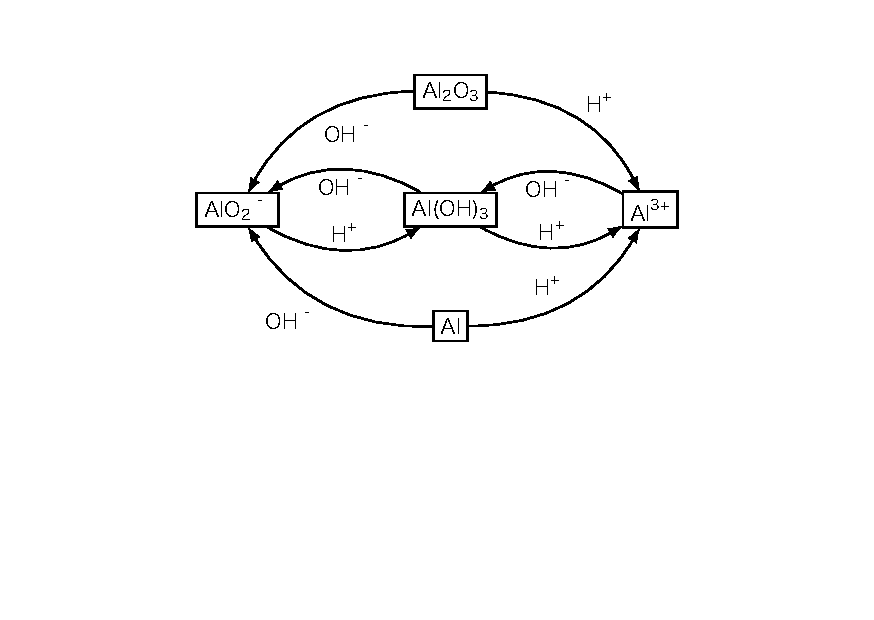
\includegraphics[scale=0.8]{res/Al.pdf}
\end{figure}